%!TEX TS-program = pdflatex
\documentclass{emulateapj}

\shorttitle{The Origin of the VOD}
\shortauthors{Casey et al}

\begin{document}

\title{The Origin of the Virgo Overdensity}

% Authors on original proposal: Stefan Keller, Andy Casey, Gary Da Costa, Daniel Zucker, Elaina Hyde, Kenji Bekki

\author{Andrew R. Casey\altaffilmark{1}, Stefan C. Keller\altaffilmark{1}, Gary Da Costa\altaffilmark{1}, Daniel Zucker\altaffilmark{2}, Elaina Hyde\altaffilmark{2}, \and Kenji Bekki\altaffilmark{3}}
\altaffiltext{1}{Research School of Astronomy \& Astrophysics, Australian National University, Mount Stromlo Observatory, via Cotter Rd, Weston, ACT 2611, Australia; acasey@mso.anu.edu.au}
\altaffiltext{2}{Department of Physics \& Astronomy, Macquarie University, Sydney 2109, Australia}
\altaffiltext{3}{ICRAR M468, The University of Western Australia, 35 Stirling Highway, Crawley, Western Australia 6009, Perth, Australia}

\begin{abstract}
\end{abstract}

\keywords{Galaxy: halo, structure --- Individual: Virgo Overdensity --- Stars: K-giants}

\section{Introduction}
%Accretion has played a vital role in the formation of the Galaxy. Consistent with the hierarchical framework of \citet{Searle;Zinn_1978}, star clusters conglomerate together to form large-scale structures like the Milky Way. 

%During later mergers, dwarf spheroidals and globular clusters experience tidal stresses during their infall. These stresses cause the perimeter stars to become unbounded from their parent cluster, and a stream of stars lie in its wake.

%The number of recent and ongoing mergers detected has increased dramatically in the wake of large sky surveys. We are only starting to realise the rich level of substructure within the galactic halo.
 

One of the most prominent of these substructures is the Virgo Overdensity (VOD). The VOD is a diffuse overdensity of stars, which is greatly dispersed along the line of sight. The VOD represents the most complex, accretion-dominated volume in the Milky Way. It is a junction for overlapping stellar streams of distinct origins \citet{Belokurov;et-al_2006}, which further complicates the task of assigning membership to stars in this region. This has also made the nature of the VOD particularly difficult to interpret: Are we witnessing the remnant of an early minor merger in the formation history of the Galaxy? Is the spatial overdensity simply an observational consequence of overlapping stellar streams? Or, is the VOD distribution smooth, and an inevitable consequence of a triaxial dark matter halo? We seek to untangle this region and address these questions.


The QUEST survey \citet{Vivas;et-al_2001} first observed an overdensity of RR Lyrae stars in this region (see also \citet{Zinn;etal_2004}). \citet{Newberg;et-al_2002} independently identified a diffuse overdensity of turnoff stars $r_\odot \sim18$ kpc away in the same direction. At the time, no relationship between these clumps could be examined. In fact, the sheer size of the VOD could not be appreciated until \citet{Juric;et-al_2008} examined the halo stellar density in the Sloan Digital Sky Survey \citep[hereafter SDSS]{York;et-al_2000} data release. \citet{Juric;et-al_2008} described the VOD as spanning well over $1,000$ deg$^{2}$ on the sky. Angular size measurements of the VOD have remained lower limits even as more data becomes available \citep{Duffau;et-al_2006, Juric;et-al_2008, Bonaco;et-al_2012}, as the substructure extends further south past the SDSS boundary. It is likely the full perimeter of the VOD will not be explored until the SkyMapper telescope \citep{Keller;et-al_2007} images this region.

The nature of the VOD is particularly important. There have been multiple kinematically cold stellar streams detected within the VOD. This strongly suggests the VOD is associated with at least one of these accreted substructures. Although the spatial overdensity is rich with substructure, it does not preclude the possibility that the overdensity is galactic in origin. Such a result which would be strong evidence for a triaxial dark matter halo \citep{Newberg;et-al_2007}. Substructures like the VOD and the Sgr tidal tails are excellent tracers of the galactic potential \citep{Law;et-al_2005, Casey;et-al_2012a}.

%The most prominent of these interacting stellar streams is the Sagittarius (Sgr) stream, which \citet{} argue is responsible for the spatial overdensity in Virgo. Who disagreed?

%As this region overlaps with several co-moving groups, it is difficult to distinguish stellar streams and halo contaminants from true VOD members. Stellar streams are somewhat easier to identify because they demonstrate a tight kinematic signature which persists for long timescales.  Table \ref{tab:vod-streams} compiles all of the published  indicators of substructure in this region. 



% what streams are running through this region

% kinematics of streams; is the VOD distinct from 

% metallicity of streams;



% origin remains debateable
There is no conclusive literature regarding the origin of the VOD, or the relationship between the spatial overdensity and the multiple kinematic signatures. Unfortunately, distances are not precise enough to help untangle the region. The uncertainty in distance for the VSS and the line-of-sight distance dispersion for the VOD has led some authors to infer they are part of the same substructure\citet{Duffau;et-al_2006, Newberg;et-al_2007, Prior;et-al_2009a}. With this hypothesis, given the low metallicities of the VSS \citep{Duffau;et-al_2006, Prior;et-al_2009a} and the wide range of metallicities present in the VOD \citep{Juric;et-al_2008}, many groups \citep{Duffau;et-al_2006, Martinez-Delgado;et-al_2007, Juric;et-al_2008} to conclude we are witnessing the tidal debris of a disrupted dwarf spheroidal (dSph) galaxy of low metallicity.


\citet{Martinez-Delgado;et-al_2007} suggest this invading dwarf is the prominent Sagittarius (Sgr) dSph galaxy. If this hypothesis is correct, the tidal debris would pass through the solar neighbourhood, providing an excellent test for the presence of weakly interacting massive dark matter particles. \citet{Martinez-Delgado;et-al_2007} predicted highly negative velocities for VOD members in this region. This signature was not observed by \citet{Newberg;et-al_2007}, implying that the VOD is distinct from the tidal debris of Sgr. However, this does not exclude the possibility of the VOD originating from a different dSph.

We present spectroscopic observations of MANY K-type stars across nineteen discretely sampled fields in the known VOD DR7 footprint \--- which was the most recent at the time of the proposal. In \S{sec:candidate-selection} we describe the candidate selection employed to minimise contamination of foreground dwarfs. Section \ref{observations} provides details of the observations taken and the data reduction method. We provide an extensive description of our spectral analysis in \S\ref{sec:spectral-analysis}, including the model atmospheres, line lists and code employed to perform these analyses. Our adopted analysis technique is verified against a plethora of spectroscopic standards in \S\ref{sec:calibration}. The data is outlined in \S\ref{sec:data} and we discuss our findings in \S\ref{sec:discussion}. We conclude in Section \ref{sec:conclusion} with critical interpretations, and outline future work necessary for this region.

\section{Candidate Selection}
We have targeted K-type giants throughout the known footprint of the VOD. These stars allow for accurate radial velocity measurements and a metallicity determination which is unbiased by their spectral type. However, colour selections employed for K giants are generally contaminated by faint, nearby dwarfs. We have taken every step to reduce this contamination, beginning with our initial colour selection.

% talk about colour selection
% 2mass and sdss, isochrone, probability, ppmxl

Some K-type dwarfs will inevitably reach into our sample. We can largely discard these contaminants with accurate surface gravity determination (see \S\ref{sec:calibration}). With our candidate selection described above, we estimate a dwarf contamination rate of approximately twenty percent.

\section{Observations and Data Reduction}
\subsection{Observations}
We present nineteen fields covering the confirmed extent of the VOD within the SDSS DR7 footprint, as illustrated in Figure \ref{fig:target-fields}. Table \ref{tab:target-fields} lists the positions, seeing, median airmass and number of stars targeted for all of our fields. 

\begin{figure}[h!]
	\includegraphics[width=\columnwidth]{./figures/fields.pdf}
	\caption{A northern Galactic cap polar plot showing the density of F turnoff stars (where $0.2 < (g - r)_0 < 0.3, (u - g)_0 > 0.4$ and $20.0 < g_0 < 21.0$) as selected by \citet{Newberg;et-al_2007}. Darker regions indicate a higher density of turnoff stars. The Sgr leading stream is evident, as is the broad extent of the VOD. The positions of our nineteen fields are shown.
	}
	\label{fig:target-fields}
\end{figure}

Observations were undertaken in normal visitor mode using the AAOmega instrument on the 3.9 m Australian Astronomical Telescope (AAT) in Coonabarabran, NSW during April 2011. The AAOmega 2dF system is a fibre-fed, dual-beam multiplexing spectrograph with interchangeable VPH gratings. AAOmega is capable of simultaneously observing 400 targets over a two degree field. The VPH gratings used were the 1500V and 1700D in the blue and red arm respectively. The 1500V grating provides a spectral coverage from $425-600$ nm at a resolution of $R \simeq 3,700$. The central wavelength for the blue arm was set to $475$ nm to prevent the gravity-sensitive Mg I b triplet lines at $\sim517$ nm falling on defective regions of the detector. The 1700D grating in the red arm provides moderate resolution ($R \simeq 10,000$) over the wavelength range $830-900$ nm, which includes the strong Ca II NIR triplet lines.

Thirty sky fibres were allocated in each field to allow for optimal sky subtraction, and a minimum of six fibres were allocated to bright stars for guiding. 

\begin{deluxetable}{cccccc}
\tablecolumns{1}
\tablewidth{\columnwidth}
\tabletypesize{\scriptsize}
\tablecaption{Field centroids and observational data\label{tab:target-fields}}
\tablehead{
	\colhead{Field} &
	\colhead{$\alpha$} &
	\colhead{$\delta$} &
	\colhead{Science} &
	\colhead{Median} &
	\colhead{Seeing} \\ 
 & (J2000) & (J2000) & Targets & Airmass & (")
}
\startdata
1 & 12 45 34  & $-$02 50 15 & 353 & 1.14 & 1.5 \\
2 & 12 46 18  & +01 09 30 & 350 & 1.24 & 1.5 \\
3 & 12 47 01  & +05 09 14 & 350 & 1.31 & 1.5 \\
4 & 12 47 46  & +09 09 01 & 324 & 1.34 & 1.5 \\
5 & 12 44 50  & $-$06 49 58 & 351 & 1.10 & 1.5 \\
6 & 12 44 06  & $-$10 49 44 & 353 & 1.49 & 1.5 \\
7 & 12 43 20  & $-$14 49 31 & 350 & 1.07 & 1.5 \\
8 & 13 09 42  & +00 29 09 & 351 & 1.30 & 1.5 \\
9 & 13 08 32  & +04 30 01 & 349 & 1.27 & 1.5 \\
10 & 13 09 35 & $-$02 33 04 & 352 & 1.39 & 1.5 \\
11 & ? & ? & ? & ? & ? \\
12 & ? & ? & ? & ? & ? \\
13 & 12 57 35 & $-$02 50 02 & 353 & 1.87 & 1.5 \\
14 & 12 33 36 & $-$02 33 41 & 350 & 1.20 & 1.5 \\
15 & 12 34 57 & +01 25 54 & 352 & 1.25 & 1.5 \\
16 & 12 36 33 & +05 24 58 & 349 & 1.31 & 1.5 \\
17 & 12 25 12 & +04 59 45 & 351 & 1.64 & 1.5 \\
18 & 12 22 48 & +01 01 10 & 352 & 1.30 & 1.5 \\
19 & 12 20 54 & $-$02 43 55 & 349 & 1.72 & 1.5 
\enddata
\end{deluxetable}

% http://www.briancasey.org/artifacts/astro/airmass.cgi

\subsection{Data Reduction}
The data was reduced using the supplied 2\textsc{DFDR} package (April 2009 version). Each frame was flat-fielded and wavelength calibrated from flat and arc frames taken between each exposure. Throughput calibration for each fibre was achieved using the night sky lines, and the sky spectrum was removed using the median flux of the dedicated sky fibres. Three twenty minute object frames were median combined to remove cosmic rays.

% speak about SNR

\section{Spectral Analysis}
\label{sec:spectral-analysis}

Stellar parameters for all of our observations were determined using the Spectral COmparison and Parameter Evaluation (SCOPE) package, which will be fully described in a later contribution \citep{Casey;et-al_2012d}. SCOPE normalises all our observations, performs doppler corrections and determines stellar parameters in an iterative manner.

\subsection{Normalisation}
Correct determination of the continuum is crucial to estimating the stellar parameters. The normalisation technique used must be sufficiently robust in noisy signals or in the presence of molecular bands, where the continuum determination can be non-trivial. A synthetic template of a typical halo giant ($T_{eff} = 4500$ K, $\log{g} = 2.5$ dex, $[\mbox{M}/\mbox{H}] = -1.5$ dex) has been used in order to estimate continuum regions of our observed spectra.

We have defined continuum regions in the synthetic spectrum where the flux level resides between $F_i: [0.96, 1.00]$. To avoid individual pixels being described as regions of continuum, we impose a minimum width of $0.5$ \AA{} for any continuum region. No maximum continuum width is imposed.

A third order cubic spline with defined knot spacing ($15$ nm in the blue arm, $20$ nm in the red arm) is fit to all observed flux points within our determined continuum regions. The knots are placed such that the distance between outer knots and the edge of the spectrum are equal. The number of knots employed is maximised until this outer distance becomes less than half the knot spacing.

The spline is weighted by the observed flux level. The difference between the determined continuum and the observed flux is calculated, and 5-$\sigma$ deviations are clipped to avoid CCD defects or persistent cosmic rays being used to incorrectly describe the continuum. This spline-fitting process is iteratively repeated until no such deviations exist.

If the observation spectrum is particularly noisy or sufficiently more metal-rich than our initial template, then our iterative spline technique discards the edge continuum regions in the sigma clipping process. When this occurs the spline may become unbounded from the outer edge knot. To correct for this effect we divide our resultant spectrum with the perfect synthetic spectrum, and fit a low order polynomial to this shape. Only the edge effects discussed above contribute to the shape of this polynomial. This technique provides a negligible correction in high SNR observations, and ensures our normalisation is robust for even the noisiest spectrum. 

Although this normalisation process is robust, experience has shown that it systematically underestimates the level of continuum by $\sim{1-2}\%$. As a final step, we demand the median flux level in continuum regions of our normalised spectra is unity.

\subsection{Radial Velocities}
Radial velocities are measured iteratively for each observation. The reduced spectrum is initially cross-correlated between $845$ nm $< \lambda <$ $870$ nm with the same synthetic spectrum employed for normalisation. The red and blue observed orders are shifted to rest frame before any further analysis. 

After the stellar parameters have been determined, we interpolate to a synthetic template with these parameters and re-measure the radial velocity. These additional radial velocity measurements provide more realistic uncertainties, and are always consistent with our initial velocity measurements.

Heliocentric velocities have been translated to a galactocentric frame. We have adopted the circular velocity of the Local Standard of Rest (LSR) at the Sun as $220 \mbox{km s}^{-1}$ \citep{Kerr;Lynden-Bell_1986} and accounted for the Sun's peculiar motion to the LSR by using $16.5 \mbox{km s}^{-1}$ towards $l = 53^\circ$, $b = 25^\circ$ \citep{Mihalas;Binney_1981}. The corrected line-of-sight velocity is then given by,
\begin{eqnarray}
	&V_{GSR} = & V_{OBS} + 220\sin{l}\cos{b} + 16.5  \\
	& 		 &\times[\sin{b}\sin{25} + \cos{b}\cos{25}\cos{(l - 53)}], \nonumber
\label{eq:vgsr}
\end{eqnarray}
\noindent{}where $V_{OBS}$ is the heliocentric-corrected observed line-of-sight velocity. We note that published velocity peaks for this region have employed slightly different formulae to transpose their kinematics to a galactocentric frame. This will result in a systematic shift in velocities between authors \--- greater than the individual uncertainties. We will address relevant discrepancies individually later in the text.


\subsection{Grid of Synthetic Spectra}

The observed stellar parameters are determined by comparing our observations to a grid of synthetic spectra with defined values. Our grid has four dimensions: effective temperature ($T_{eff}$), surface gravity ($\log{g}$), metallicity ($[\mbox{Fe}/\mbox{H}]$) and alpha enhancement ($[\alpha/\mbox{Fe}]$). The bounds of this grid are illustrated in Figure \ref{fig:grid-boundaries}. These boundaries sufficiently extend past the expected values from our observations.

\begin{figure}[h!]
	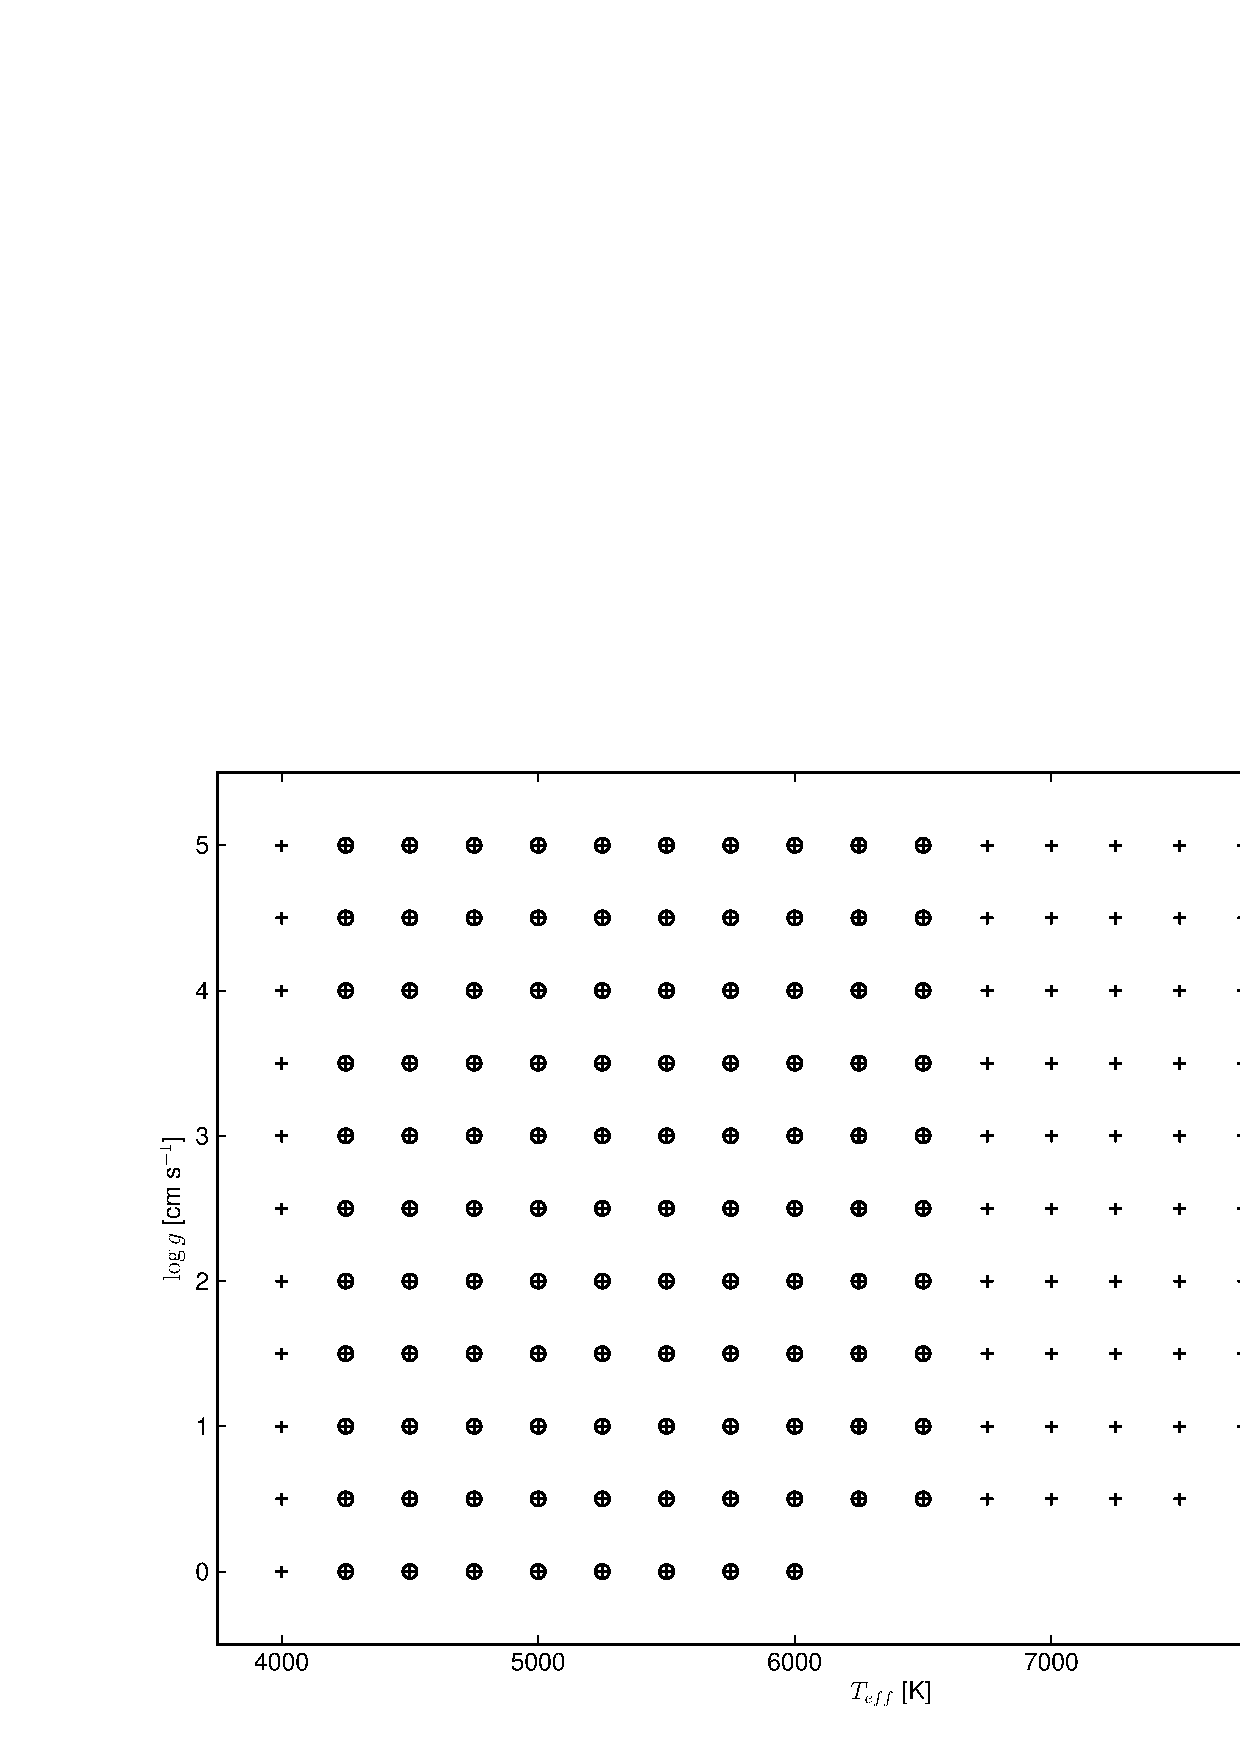
\includegraphics[width=\columnwidth]{./figures/grid-points.pdf}
	\caption{A 2D representation of our synthetic grid points. Each illustrated point has a number of metallicities: the pluses (+) indicate metallicity points between -2.5 and +0.5 dex with 0.5 dex steps and an additional point at [Fe/H] = $+0.2$ dex, and the encircled pluses (++) illustrate where we have extended our metallicity grid down to [Fe/H] = -5.5 at 0.5 dex steps. Every point has a solar-level [$\alpha$/Fe] and an alpha enhancement [$\alpha$/Fe] = +0.4 dex.}
	\label{fig:grid-boundaries}
\end{figure}




Throughout this article we refer to the metallicity ($[\mbox{Fe}/\mbox{H}]$) as the bulk metal content of heavy elements. Standard spectroscopic abundance notation is adopted such that the ratio of two elements in a star relative to their ratio in the Sun is
\begin{equation}
[\mbox{A}/\mbox{B}] \equiv \log{[n(\mbox{A})/n(\mbox{B})]} - \log{[n(\mbox{A})/n(\mbox{B})]}_\odot,
\end{equation}
\noindent{}where $n$ represents the number density. The level of alpha enhancement ($[\alpha/\mbox{Fe}]$) is quantified by the abundance of the $\alpha$-elements Mg, Si, S, Ar, Ca and Ti. These elements all vary together. 

\subsubsection{Model Atmospheres}
A model stellar atmosphere is required before a synthetic spectrum can be computed. Stellar atmosphere models tabulate pressure, temperature, electron fraction and opacity as a function of optical depth within the stellar atmosphere. We have chosen to use the \citet{Castelli;Kurucz_2004} grid of plane-parallel model atmospheres with no convective overshoot \citep{Castelli;Kurucz_1997} and updated opacity distribution functions \citep{Castelli;Kurucz_2003}. Microturbulent velocity ($v_t$) for our synthetic spectra was fixed as $2$ km s$^{-1}$.

\subsubsection{Line List}
We have compiled a line list of wavelengths, excitation potentials (EPs), and oscillator strengths ($\log{gf}$) for atomic, hyperfine and molecular transitions spanning our observed spectral range. Generally the wavelength transition locations are well known, however oscillator strengths are notoriously difficult to measure. High resolution spectroscopic analysis will typically only compare line strengths for well established transitions within the linear regime of the curve of growth. In this analysis we are considering a wide spectral range at a lower resolution, where most lines will be blended. Consequently we must use an extensive library of transitions, which will all contribute to the derived parameters with varying degree.

We began by querying the Vienna Atomic Line Database \citep[VALD][]{Kupka;et-al_1999} in March 2012 and retrieved all neutral and singular atomic transitions within the spectral ranges $380-605$ nm and $830-890$ nm with $0 < \mbox{EP} < 10.2$ eV and $\log{gf} > -5$. The list was supplemented with molecular transitions from \citet{Kurucz_1992} for the $A^2\Pi-X^{2}\Sigma$ CN and MgH transitions, and all C$_2$ transitions. Hyperfine transitions for Li, Sc, V, Mn, Co, Cu, and Eu from \citet{Kurucz_1993} were included in our list. 

SCOPE's line list calibration routine was employed to match our generated synthetic spectrum with the Solar \citep{Wallace;et-al_2011} and Arcturus \citep{Hinkle;et-al_2003} atlases. We generated spectra in MOOG \citep[see \S\ref{sec:synth-generation}]{Sneden_1973}, using a Solar atmosphere model where $T_{eff}= 5577$ K, $\log{g} = 4.437$, $[\mbox{M}/\mbox{H}] = 0.00$ and $v_{t} = 1.0$ km s$^{-1}$. The synthetic spectrum was matched to the atlas dispersion and convolved with a $0.05$ dex wide Gaussian kernel.

We chose to perform our line calibration interactively on selected line discrepancies instead of using a completely automatic approach. Beginning with the strong line transitions, the oscillator strength of each line is varied and the $\chi^2$ statistic (variant of Eq. \ref{eq:chi}) between the synthetic spectrum and the observed atlas is calculated. The Nelder-Mead optimisation algorithm \citep{Nelder;Mead_1965} was employed to determine the oscillator strength and minimise the $\chi^2$ value. We iterated until a $10^{-4}$ relative change in $\log{gf}$ was achieved. When the transition in question belongs to a multiplet, we alter the relative oscillator strength for all transitions in the multiplet simultaneously. It is worth noting that although we found a much better statistical fit when altering each transition individually, this is forbidden by quantum mechanics.

We repeated this process for the discrepant weaker transitions. Our revised strong line list was employed and the relative oscillator strength was varied for lines in the weaker multiplets. When we observed an absorption feature not present in our line list, we invented a Fe transition with the required excitation potential and oscillator strength to replicate the observed profile. Using this calibration technique the median absolute RMS between our synthetic spectrum and the Sun has decreased from $1.3 \times 10^{-3}$ to Y, and the deviation from $9.3 \times 10^{-2}$ to B.

This calibration process was repeated on the Arcturus atlas of \citet{Hinkle;et-al_2003}. We used a depth-varying atmospheric model for Arcturus \citep{Kurucz}, where $T_{eff} = X, \log{g} = X, [\mbox{Fe}/\mbox{H}] = 0.00$. Taking the Solar atlas to be more precise and the Solar atmosphere to be better modelled, we only used Arcturus-calibrated oscillator strengths if they did not increase the $\chi^2$ value in the equivalent Solar spectrum. The mean absolute RMS of our fit lowered from $X \pm Y$ (using the Solar-calibrated line list) to $Z \pm A$ through this technique. The entirety of our line list is published in Table \ref{tab:line-list}.


\begin{deluxetable}{cccc}
\tablecolumns{1}
\tablewidth{\columnwidth}
\tablecaption{List of transition lines\label{tab:line-list}}
\tablehead{
	\colhead{Wavelength} &
	\colhead{Species} &
	\colhead{EP} &
	\colhead{$\log{gf}$} \\ 
	(\AA) & & (eV) & (dex)
}
\startdata
8300.229 & 25.0 & 6.752 & -2.602 \\
8300.229\tablenotemark{a} & 25.0 & 6.752 & -2.602 \\
8300.229 & 25.0 & 6.752 & -2.602 \\
8300.229\tablenotemark{b} & 25.0 & 6.752 & -2.602 \\
\enddata
\tablenotetext{a}{Invented transition to match atlas.}
\tablenotetext{b}{Strong transition.}
\end{deluxetable}


\subsubsection{Synthetic Spectrum Generation}
\label{sec:synth-generation}
The synthetic spectrum for each grid point has been generated using MOOG. We have employed \citet{Anders;Grevesse_1989} solar abundances, with the exception of Fe, where we have used the revised value from \citet{Asplund;et-al_2005}. The absorption caused by stronger transitions was considered at every wavelength step. In the blue arm, the strong lines include the Ca H, Ca K, and Mg I b triplet lines at $\lambda517$nm. For the red arm these lines include the Ca II NIR triplet lines, and Na I at $\lambda8807$. The absorption contribution for all weaker transitions was considered within $2$ \AA{} of their core depth. 

The spectra was generated at a resolution of $0.10$ \AA{} px$^{-1}$, and is later re-sampled to match the observed wavelength-pixel dispersion and convolved to match our resolving power.

\subsection{Stellar Parameter Determination}

SCOPE determines stellar parameters by minimising the $\chi^2$ value,
\begin{equation}
\chi^2 = \frac{1}{N-M}\sum\limits_{i=0}^{N}\frac{(F_i - f_i)^2}{\sigma_i}
\end{equation}
\noindent{}where the synthetic and observed flux is represented by $F_i$ and $f_i$ respectively, $M$ is the number of degrees of freedom (e.g. $T_{eff}$, $\log{g}$, $[\mbox{Fe}/\mbox{H}]$, $[\alpha/\mbox{Fe}]$), and the uncertainty $\sigma_i$ is measured from $(\mbox{S}/\mbox{N})^{-2}$.

Observations are compared against the grid of synthetic spectra and a $\chi^2$ value is determined at every grid point. This sampling technique is a relatively expensive computational step, but it is necessary to confidently prevent false positive determinations of atmospheric parameters. There are techniques available within SCOPE to minimise the level of sampling required (see \S\ref{sec:effective-temperature}).

When the grid sampling is completed a subset of points surrounding the minimum $\chi_{min}^2$ point are used for flux interpolation. Because our observed parameters do not reside on evenly spaced grid points, interpolation within the synthetic grid of fluxes is necessary. We linearly interpolate in flux space \--- not $\chi^2$ space \--- such that our synthetic flux becomes a continuous function within the grid boundaries. One-dimensional splines are fit to the minimum along each axis, and an estimate of the inter-grid $\chi^2$ minima is provided as an initial guess to a Nelder-Mead optimising algorithm (see Figure \ref{fig:chi-estimate}). Points within the entire subset are sampled until the minima is found and a $10^{-8}$ tolerance in $\chi^2$ is achieved. 

% Figure showing chi^2 sampling and a spline estimate, then the optimisation.


\subsubsection{Photometric temperature estimates}
\label{sec:photometric-estimates}

All of our observations were cross-matched against the 2MASS catalogue prior to analysis and a photometric temperature is calculated. Photometric estimates of stellar parameters can be used to restrict the level of synthetic grid sampling required. We have adopted the empirical $T_{eff}$-colour relationship for F0-K5 giant stars from \citet{Alonso;et-al},
\begin{equation}
\theta_{eff} = 0.5816 + 0.9134(J-K)_0 - 0.1443(J-K)_{0}^2
\end{equation}

\noindent{}where $T_{eff} = 5040/\theta_{eff}$. The dust maps of \citet{Schlegel;et-al_1998} with revised bandpasses from \citet{Schonrich;et-al_2011} were used to correct for interstellar extinction. Because we are constraining the range of temperature points sampled in our synthetic grid, it is of critical importance not to underestimate the uncertainty in this relationship. \citet{Alonso;et-al} report an uncertainty of $125$ K using this relationship. We have pessimistically included the photometric uncertainties ($\sigma_J$, $\sigma_K$) to estimate a photometric contribution to the total error budget as,
\begin{equation}
\sigma_{phot} = T_{eff}(J_0+\sigma_J - K_0 +\sigma_K) - T_{eff}(J_0 - K_0)
\end{equation}

\noindent{}and added these two error sources in quadrature. The synthetic grid is restricted by 3-$\sigma_{total}$ either side of the photometric temperature (typically this equates to $\sim\pm1,200$ K). In extremely rare cases when the grid has been photometrically constrained and the spectroscopically determined temperature was close to the edge of the restricted grid, the photometric constraint was removed and the analysis was repeated.

\subsubsection{Solution steps}
\label{sec:solution-steps}

SCOPE allows us to set up any number of solution steps, where we can solve for atmospheric parameters either individually or any number of them simultaneously. After extensive testing, we have adopted a recipe which solves for $T_{eff}$, $[\mbox{Fe}/\mbox{H}]$, and $[\alpha/\mbox{Fe}]$ first simultaneously, and then solves for $\log{g}$. Different wavelength regions are used for the $\chi^2$ evaluation in each solution step. These comparison regions are tabulated in Table \ref{tab:solution-setup}.

% table here showing entire comparison regions
% Dimension(s) | Regions 

\begin{deluxetable}{ccccc}
\tablecolumns{1}
\tablewidth{\columnwidth}
\tablecaption{SCOPE solution setup.\label{tab:solution-setup}.}
\tablehead{
& Measured & Fixed & \multicolumn{2}{c}{Regions} \\
	\colhead{Step} &
	\colhead{Parameters} &
	\colhead{Parameters} &
	\colhead{$\lambda_a$} &
	\colhead{$\lambda_b$} \\
	& & & (\AA{}) & (\AA{})
}
\startdata
1 & $T_{eff}, [\mbox{Fe}/\mbox{H}], [\alpha/\mbox{H}]$ & None & 8400.0 & 8850.0 \\
&&& 8400.0 & 8850.0 \\
 2 & $\log{g}$ & $T_{eff}, [\mbox{Fe}/\mbox{H}]$ & 8400.0 & 8850.0
\enddata
\end{deluxetable}


\subsubsection{Metallicity, $[\mbox{Fe}/\mbox{H}]$}
We solve for metallicity and temperature simultaneously. After extensive testing we determined that the known degeneracies between $T_{eff}-[\mbox{Fe}/\mbox{H}]$ are simply too prominent in our data to allow for solving $T_{eff}$ and [Fe/H] separately. 




\subsubsection{Alpha Abundance, $[\alpha/\mbox{Fe}]$}

\begin{equation}
[\alpha/\mbox{Fe}] = [\alpha/\mbox{H}] - [\mbox{Fe}/\mbox{H}]
\end{equation}

\subsubsection{Surface Gravity, $\log{g}$}
We solve for surface gravity in our second solution step. During this step we only use the $516-519$ nm region surrounding the Mg I b triplet lines for comparison. The $\chi^2$ statistic has a tendency to be influenced by regions of the spectrum which are not sensitive to atmospheric parameters. This is typically nor a problem for $T_{eff}$ and [Fe/H] because large regions of the spectrum are sensitive to these parameters. Given the difficulty in measuring surface gravity, we have chosen only to use a region which we know is particularly gravity sensitive.

Tests performed with SCOPE have indicated that if $T_{eff}$ is not fixed when measuring $\log{g}$ then the $\chi^2$ space is not sufficiently well-described in order to find the true surface gravity. Multiple local minima are present; an incorrect initial guess is often provided to our optimisation algorithm. We also noticed a strong degeneracy present between [Fe/H] and $\log{g}$: if [Fe/H] is fixed to the value we have determined in the previous solution step, then then our surface gravity measurements incur significant scatter. Hence, when measuring surface gravity we fix the temperature to the value we have previously determined, and allow [Fe/H] to be free.

\section{Verification of analysis technique}
\label{sec:calibration}

We have validated our analysis technique with three different data sets: two high resolution spectroscopic libraries with exquisite S/N, and RGB stars in ten globular clusters observed on the AAT.

\subsection{Spectroscopic Libraries}
There is a growing number of high resolution spectroscopic libraries available for comparison, however few of them cover the spectral range covered by AAOmega's 1500V/1700D filter set.

\label{sec:S4N}
\subsubsection{The S$^4$N Library}
The S${^4}$N library contains high resolution, high S/N spectroscopic observations of 118 stars within the Solar neighbourhood \citep{Allende-Prieto;et-al_2004}. These observations cover a wide wavelength range from $\sim362$ nm to $921$ nm with a resolving power of $R\simeq50,000$. Published spectra are already normalised and placed at rest frame. Thus, we chose not to re-normalise the spectra or apply doppler corrections.

The S$^4$N observations were interpolated to the same pixel-dispersion map as our observations, and convolved to match our resolving power. The S/N for the S$^4$N spectra varies between $150-600$. Resampling these observations adds correlated noise, albeit negligible in this case. Hence we are now effectively working with medium resolution observations with exceptional S/N. We have chosen not to add additional shot noise for this initial comparison \--- the effects of Poisson noise are examined later in \S\ref{sec:shot-noise}.

\begin{figure*}[t!]
	\includegraphics[width=\textwidth]{./figures/s4n-comparison.pdf}
	\caption{Comparison between the determined atmospheric parameters for the S$^{4}$N stellar catalogue at high resolution \citep{S4N}, and the values determined after resampling and convolving the spectra to our observed dispersion and resolution. The dashed lines indicate 1\---$\sigma$ deviations between the expected and determined parameters.}
	\label{fig:s4n-comparison}
\end{figure*}


Discrepancies between the expected atmospheric parameters of \citet{Barklem;et-al_2004} and derived values are illustrated in Figure \ref{fig:s4n-differences}. We recover atmospheric parameters with excellent precision. The 1\---$\sigma$ dispersions in $T_{eff}$, $\log{g}$ and $[\mbox{Fe}/\mbox{H}]$ correspond to $205$ K, $0.40$ dex and $0.15$ dex respectively. These values are tabulated with our CFLIB discrepancies in Table \ref{tab:grid-boundaries}, and are typical uncertainties for spectra at this dispersion and resolution.

% see allende-prieto re IRFM -- Blackwell

\subsubsection{CFLIB}
\label{sec:CFLIB}
Although our S$^4$N comparative results are encouraging, the S$^4$N stars are all solar neighbourhood dwarfs and do not represent our target selection. In fact, they more closely represent our contaminants. We have performed the same analysis on the CFLIB library \citep{Valdes;et-al_2007}, which includes both giants and dwarfs. The atmospheric parameters reported for CFLIB come from a variety of literature sources; the analysis technique was not homogenous. Compared to S$^4$N, we can expect a larger dispersion in these results.

Most CFLIB spectra extends from $346$ nm to $964$ nm. Multiple exposures with different grating configurations are required to cover this full spectral range and consequently some observations have only partial wavelength coverage. We excluded observations which did not have coverage across our $\chi^2$ comparison regions. Observations with expected parameters outside of our synthetic grid boundaries were also discarded.

% Instead of using the single measurements compiled by \citet{Valdes;et-al_2004} as our expected parameters, we queried the PASTEL database \citep{Soubiran;et-al_2010} for all the CFLIB stars with multiple measurements of the stellar parameters. We excluded observations where only one determination of the stellar parameters was available, or if the published parameters were wildly inconsistent. Our distilled sample size of CFLIB spectra is 361 stars \--- including 188 giants and 173 dwarfs (separated by $\log{g} = 3.5$).

% num covering spectral regions: 800 (spectra)

% JUST ON PASTEL
% num with 2+ measurements in all dimensions: 646 (multi)
% num within grid: 671 (inbounds)
% num with [fe/h] < -1 (mp): 90
% intersection of (inbounds) & (multi | mp): 611 (total)

% WITH SPECTRAL RANGE INCL.
% intersection of (total) & (spectra): 438
% multiple measurements: 386 (multi)18
% in bounds: 392 (in_bounds)
% mp: 24 (mp)
% usable (in_bounds) & | ((multi_measured) | (mp)): 361
% giants (logg < 3.5) in (usable): 188
% dwarfs (logg >= 3.5) in (usable): 173


% Include figure for CFLIB results

\begin{deluxetable}{lccc}
\tablecolumns{1}
\tablewidth{\columnwidth}
\tablecaption{Biases and dispersions for derived parameters in existing high resolution libraries.\label{tab:hrs-comparison}}
\tablehead{
	 &
	\colhead{$T_{eff}$} &
	\colhead{$[\mbox{Fe}/\mbox{H}]$} &
	\colhead{$\log{g}$} \\ 
	 & (K) & (dex) & (cm s$^{-1}$)
}
\startdata
S$^{4}$N (all stars) & $33 \pm 190$ & $0.02 \pm 0.15$ & $-0.04 \pm 0.35$ \\
CFLIB (dwarfs)\tablenotemark{a} & & & \\
CFLIB (giants)\tablenotemark{a} & & & \\
CFLIB (all stars) & & &
\enddata
\tablenotetext{a}{For this comparison, we separate giants and dwarfs at $\log{g} = 3.5$ dex.}
\end{deluxetable}

% Discuss CFLIB comparison values and any systematic offsets between dwarfs/giants and perhaps MPG/MPD/MRG/MRD


\subsection{Globular Clusters}
\label{sec:globular-clusters}
The CFLIB and S$^4$N spectral libraries provide an excellent way to verify our analysis technique against atmospheric parameters determined by excitation and equilibrium balances. Although they were resampled and convolved to match our observed conditions, ultimately they were not observed on the AAT. As a final verification of our technique we observed red giant stars in multiple globular clusters to compare kinematics and stellar parameters.

Observed globular clusters are tabulated in Table \ref{tab:globular-clusters} with their relevant properties \citep{Harris}. 

% median metallicities

% tabulated values of stuff employed (age, feh, etc)
% name (alt name), Age, v_helio, harris v_helio, feh, harris feh, No. stars

 


\begin{deluxetable}{lcccccc}
\tablecolumns{1}
\tablewidth{\columnwidth}
\tablecaption{Observed cluster median metallicities and kinematics.\label{tab:globular-clusters}}
\tablehead{
	\colhead{Cluster} &
	\colhead{Age} &
	\colhead{$V_{helio,ARC}$} &
	\colhead{$V_{helio,HARRIS}$} &
	\colhead{feh} &
	\colhead{feh} &
	\colhead{vmvhb} 
}
\startdata
\enddata
\tablenotetext{a}{For this comparison, we separate giants and dwarfs at $\log{g} = 3.5$ dex.}
\end{deluxetable}


% isochrones and points for every cluster


\subsection{The effects of shot noise}
\label{sec:shot-noise}
We have employed the S$^4$N library to examine the affect of Poisson shot noise on our derived stellar parameters. All S$^4$N spectra were analysed with four levels of S/N: 15, 30, 50 and 100 px$^{-1}$. The $1\--\sigma$ dispersions in derived stellar parameters are illustrated in Figure \ref{fig:shot-noise} and tabulated in Table \ref{tab:shot-noise}. No significant biases in derived stellar parameters were found with increased Poisson noise.

\begin{deluxetable}{cccc}
\tablecolumns{1}
\tablewidth{0pt}
\tabletypesize{\scriptsize}
\tablecaption{Dispersion in derived stellar parameters for S$^4$N stars with artificial shot noise.\label{tab:shot-noise}}
\tablehead{
	\colhead{S/N} &
	\colhead{$T_{eff}$} &
	\colhead{$\log{g}$} &
	\colhead{$[\mbox{M}/\mbox{H}]$} \\ 
	(px$^{-1}$) & (K) & (dex) & (dex)
}
\startdata
100 & 0 & 0 & 0 \\
50 & 0 & 0 & 0 \\
30 & 0 & 0 & 0 \\
15 & 0 & 0 & 0 
\enddata
\end{deluxetable}

% confident that our analysis is valid
% confident down to a certain SNR, at which point below this value we will not use derived parameters?



The analysis procedure described in S\ref{sec:calibration} was applied to all 10,232 spectroscopic observations.



\section{Data Quality}

We carefully inspected both beam of every normalised observation and its best-fitting synthetic fit prior to interpreting our results. During this process we uncovered 2 typical carbon stars and identified sub-optimal normalisation for 35 objects. There were 35 spectroscopic binaries were discarded from further analysis, as well as 832 other observations with indecipherable signal. Observations with incorrect continuum determination were  interactively re-normalised using the same process described in \S\ref{sec:normalisation} with slightly varied constraints on sigma clipping and spline knot placement.


Stellar parameters derived from observations with a S/N below 20 are uncertain and have not been published. An upper limit on $\chi^2$ has not been placed. However, we visually inspected every observation with a $\chi^2$ value greater than FOUR?. These unusually high $\chi^2$ values are ubiquitously attributable to bad columns in our comparison regions. After inspecting our data for quality assurance, our distilled sample of results is 9,820 K-type stars \--- roughly X\% were excluded.

% SNR vs V_err? 
% SNR vs chi^2
% fibre number and chi^2 to illustrate effect of bad columns?

\section{Results}
\label{sec:results}



\section{Discussion}
\label{sec:discussion}


\section{Conclusions}
\label{sec:conclusions}

\section{Acknowledgements}
\label{sec:acknowledgements}

ARC is pleased to acknowledge the financial support through the Australian Research Council Laureate Fellowship 0992131.  SK and GDaC acknowledge the financial support from the Australian Research Council through Discovery Program DP0878137.

This publication makes use of data products from the Two Micron All Sky Survey, which is a joint project of the University of Massachusetts and the Infrared Processing and Analysis Center/California Institute of Technology, funded by the National Aeronautics and Space Administration and the National Science Foundation.

Funding for the SDSS and SDSS-II has been provided by the Alfred P. Sloan Foundation, the Participating Institutions, the National Science Foundation, the U.S. Department of Energy, the National Aeronautics and Space Administration, the Japanese Monbukagakusho, the Max Planck Society, and the Higher Education Funding Council for England. The SDSS Web Site is http://www.sdss.org/.

The SDSS is managed by the Astrophysical Research Consortium for the Participating Institutions. The Participating Institutions are the American Museum of Natural History, Astrophysical Institute Potsdam, University of Basel, University of Cambridge, Case Western Reserve University, University of Chicago, Drexel University, Fermilab, the Institute for Advanced Study, the Japan Participation Group, Johns Hopkins University, the Joint Institute for Nuclear Astrophysics, the Kavli Institute for Particle Astrophysics and Cosmology, the Korean Scientist Group, the Chinese Academy of Sciences (LAMOST), Los Alamos National Laboratory, the Max-Planck-Institute for Astronomy (MPIA), the Max-Planck-Institute for Astrophysics (MPA), New Mexico State University, Ohio State University, University of Pittsburgh, University of Portsmouth, Princeton University, the United States Naval Observatory, and the University of Washington.

\bibliographystyle{apj}
\bibliography{bibliography}


\end{document}